% !TEX program = xelatex
\documentclass{article}

\usepackage{mathtools}
\usepackage{amssymb}
\usepackage{unicode-math}
\setmonofont{DejaVu Sans Mono} % monospaced font with extensive unicode support for verbatim
\usepackage{stmaryrd}
\usepackage{booktabs}
\usepackage{tikz}
\usepackage{forest}
\usepackage{logicproof}
\usepackage{ebproof}
\usepackage{fitch}
\usepackage[capitalize,noabbrev]{cleveref}
\usepackage{subcaption}
%%%%%%% Some macros to help with the typesetting %%%%%%%%%%
\usepackage{logic-macros}
%%%%%% End of local macros %%%%%%%

\title{Mathematical Structures Homework 1}
\author{Jenny Vermeltfoort\\
  s3787494\\
  Informatica%Informatica, I&E, Bioinformatica, Wiskunde, ...
}

\begin{document}

%% Use var symbols by default
\renewcommand*{\phi}{\varphi}
\renewcommand*{\epsilon}{\varepsilon}

\maketitle

\section*{Exercise 1}
a)
Degrees of freedom is four, since:
\begin{itemize}
  \item we have two angles for the base joint: one angle on the xy plane ($\Phi_{2}$), one angle on vertical ($\Phi_{1}$) plane, and one angle that depicts the rotation over the vertical axis ($\Phi_3$).
  \item the length ($d$) of the upper arm segment which is bounded on the interval $[20, 100]$.
\end{itemize} 

The configuration space $C$ is:
$C = \mathbb{R}^4 $

We project the configuration space into a Cartesian coordinate space:
$X = \mathbb{R}^3$

The transformation function $t$ defined as:
\begin{equation}
  t_a: C \rightarrow X, t_b: C \rightarrow X
\end{equation}
with $ 0 \leq \Phi_{1} \leq \frac{\pi}{2} $.
\begin{equation}
  \mathbf{A} = t_a(\Phi_{1}, \Phi_{2}, d) = \\
  d \cdot \begin{pmatrix}
    \cos(\Phi_{1}) * \cos(\Phi_{2}) \\
    \cos(\Phi_{1}) * \sin(\Phi_{2}) \\
    \sin(\Phi_{1}) \\
  \end{pmatrix}
\end{equation}

\begin{equation}
  \mathbf{B} = t_b(\Phi_{1}, \Phi_{2}, d, \Phi_{3}) = \mathbf{A} + \\
  10 \cdot \begin{pmatrix}
  \cos(\Phi_{1} + \frac{3\pi}{2}) \cos(\Phi_{2}) \cos(\Phi_{3}) \\
  \cos(\Phi_{1} + \frac{3\pi}{2}) \sin(\Phi_{2}) \cos(\Phi_{3}) \\
  \sin(\Phi_{1} + \frac{3\pi}{2}) \sin(\Phi_{3}) \\
  \end{pmatrix}
\end{equation}

\begin{figure}[h]
    \centering
    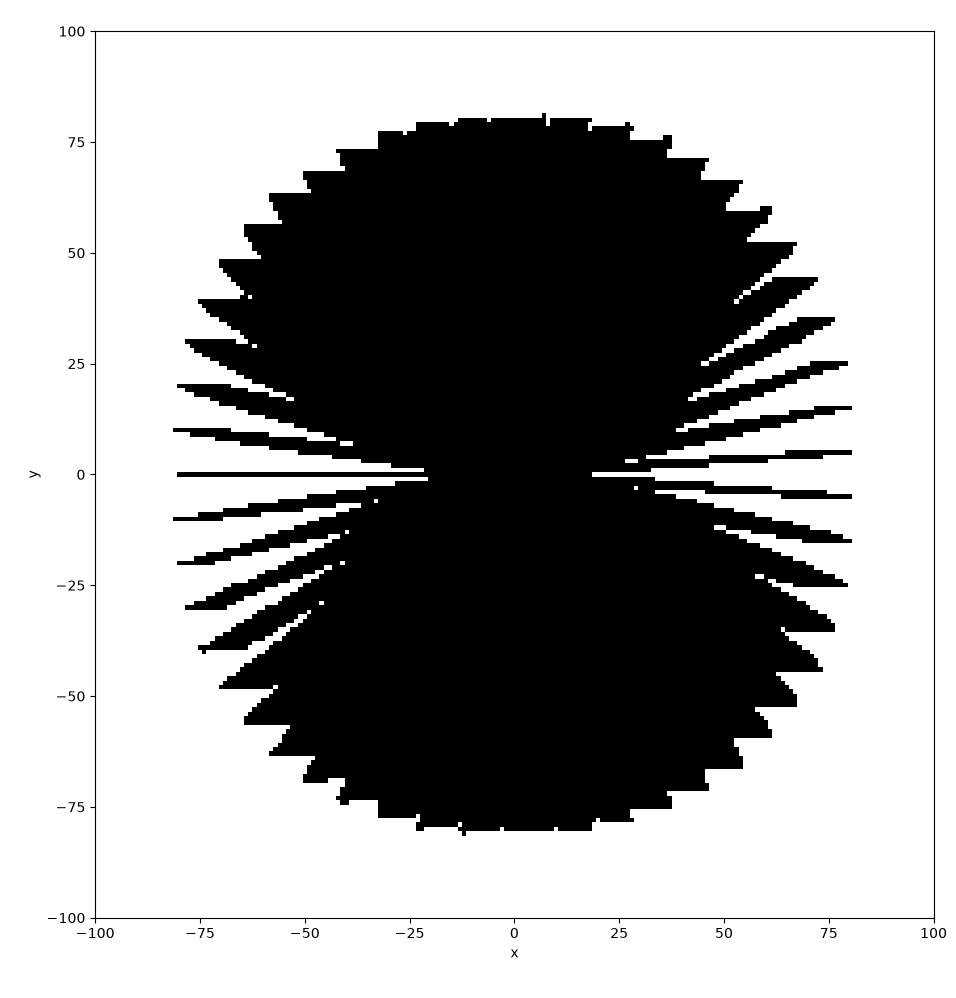
\includegraphics[width=0.75\textwidth]{Figure_1.png}
    \caption{}
    \label{fig:sample1}
\end{figure}

\begin{figure}[h]
    \centering
    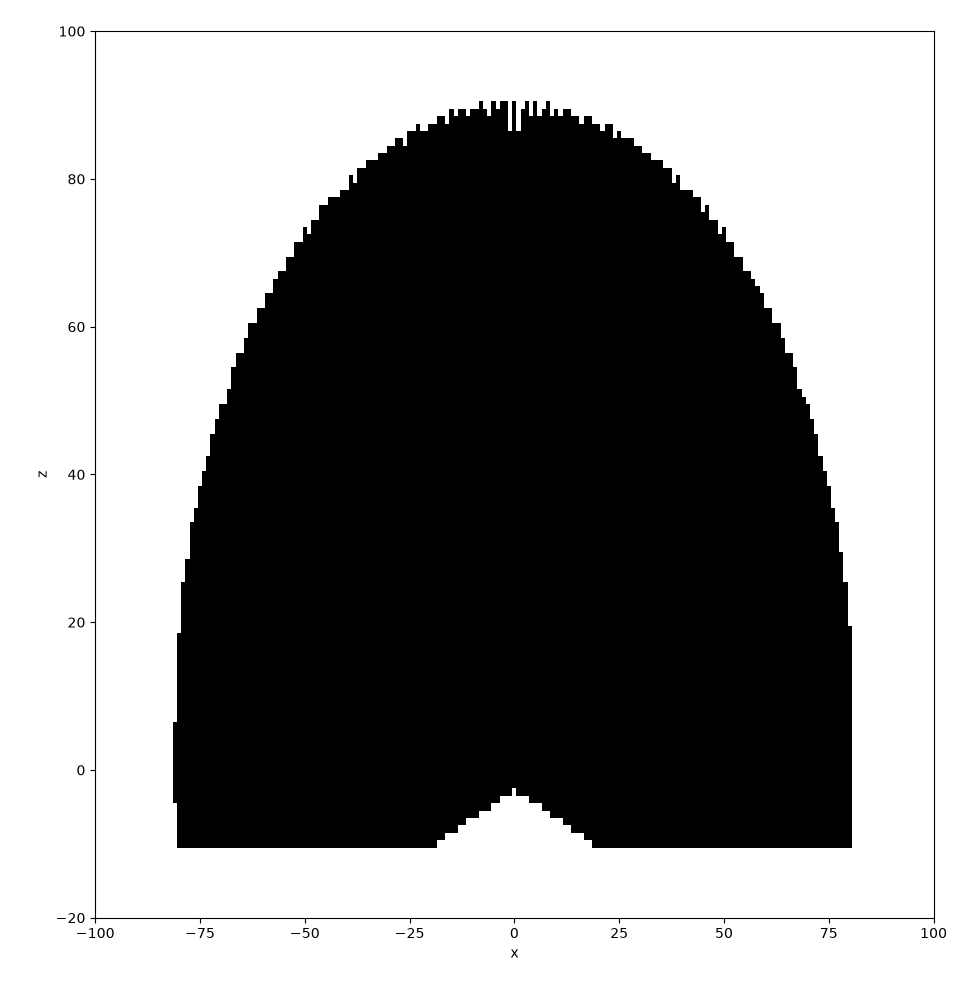
\includegraphics[width=0.75\textwidth]{Figure_2.png}
    \caption{}
    \label{fig:sample2}
\end{figure}


\newcommand\myeq{\mathrel{\stackrel{\makebox[0pt]{\mbox{\normalfont\tiny def}}}{=}}}

\section*{Question 2}

1. 
a) $u \cdot v =  0  -8  -3  = -11 $ \\
b) $ \| u \|_2 = \sqrt{14}, \| v \|_2 = \sqrt{17} $ \\
c) $ \| u \|_{\inf} = 3,  \| v \|_{inf} = 4 $ \\

2.
a) $u \cdot v = 4 -2 -6 = -4 $ \\
b) $ \| u \|_2 = \sqrt{6}, \| v \|_2 = 2\sqrt{6} $ \\
c) $ \| u \|_{\inf} = \sqrt{3},  \| v \|_{inf} = \sqrt{12} $ \\

3.
a) $u \cdot v = \cos \theta \sin \theta + \sin \theta \cos \theta  = 2 cos \theta sin \theta $ \\
b) $ \| u \|_2 = \sqrt{2}, \| v \|_2 = 1 $ \\

\section*{Question 3}

1. $ \int_{0}^{1} 3x^3 -x^2 = \left[ \frac{3}{4}x^4 - \frac{1}{3}x^3 \right]^1_0 = \frac{5}{12} $

2. $ \int_{0}^{1/2} x e^{2x} = \left[ \frac{1}{2}xe^{2x} - \frac{1}{2} \int_{0}^{1/2} e^{2x} \right]^{1/2}_0 = \left[  \frac{1}{2}xe^{2x} - \frac{1}{4}e^{2x} \right]^{1/2}_0 = \frac{1}{4} $

3. 
\begin{math}
  I = \int_{-\sqrt3}^{\sqrt(3)} cos(3x)sin(3x) dx = \frac{1}{3} \int_{-\sqrt{3}}^{\sqrt{3}} cos(t)sin(t) dt \\
  = \frac{1}{3}\sin^2(t) - \frac{1}{3} \int_{-\sqrt{3}}^{\sqrt{3}} cos(t)sin(t) dt \\
  2I = \left[  \frac{1}{3}\sin^2(t) \right]^{\sqrt{3}}_{-\sqrt{3}} \\
  I = \left[  \frac{1}{6}\sin^2(t) \right]^{\sqrt{3}}_{-\sqrt{3}} = 0
\end{math}

\section*{Question 4}
1. With $x, y \in V$
Non-negative: $ 0 \leq \| x \| $. 
Triangular equality: $ $


\end{document}